\documentclass[12pt]{article}
\usepackage{ragged2e} % load the package for justification
\usepackage{hyperref}
% to remove the hyperline rectangle
\hypersetup{
	colorlinks=true,
	linkcolor=orange!80!black, % Set the link color to blue
	urlcolor=blue,  % Set the URL color to blue
	citecolor=blue, % Set the citation color to blue
}
\usepackage{graphicx}
\usepackage{pdfcomment}

\usepackage[utf8]{inputenc}


\usepackage{pgfplots}
\usepackage{tikz}
\usepackage{pgf-pie}
\usetikzlibrary{pgfplots.statistics}


\usepackage{filecontents}
\usepackage{multirow}
\usepackage{amsmath}
\pgfplotsset{width=10cm,compat=1.17}
\setlength{\parskip}{0.75em} % Set the space between paragraphs
\usepackage{setspace}
\setstretch{1.2} % Adjust the value as per your preference
\usepackage[margin=2cm]{geometry} % Adjust the margin
\setlength{\parindent}{0pt} % Adjust the value for starting paragraph

\usepackage{mdframed}


\usepackage{xcolor}
\usepackage{titlesec}
\usepackage{titletoc}
\usepackage{listings}
\usepackage{tcolorbox}
\usepackage{lipsum} % Example text package
\usepackage{fancyhdr} % Package for customizing headers and footers



% Define the orange color
\definecolor{myorange}{RGB}{255,65,0}
% Define a new color for "cherry" (dark red)
\definecolor{cherry}{RGB}{148,0,25}
\definecolor{codegreen}{rgb}{0,0.6,0}




%%%%%%%%%%%%%%%%%%%%%%%%%%%%%%%%%%%%%%%%%%%%%%%%%%%%%%%%%%%%%%%%%%%%%
% Apply the custom footer to all pages
\pagestyle{fancy}

% Redefine the header format
\fancyhead{}
\fancyhead[R]{\textcolor{orange!80!black}{\itshape\leftmark}}

\fancyhead[L]{\textcolor{black}{\thepage}}


% Redefine the footer format with a line before each footnote
\fancyfoot{}
\fancyfoot[C]{\footnotesize P. Pasandide, McMaster University, Computer Science Practice and Experience: Development Basics. \footnoterule}

% Redefine the footnote rule
\renewcommand{\footnoterule}{\vspace*{-3pt}\noindent\rule{0.0\columnwidth}{0.4pt}\vspace*{2.6pt}}

% Set the header rule color to orange
\renewcommand{\headrule}{\color{orange!80!black}\hrule width\headwidth height\headrulewidth \vskip-\headrulewidth}

% Set the footer rule color to orange (optional)
\renewcommand{\footrule}{\color{black}\hrule width\headwidth height\headrulewidth \vskip-\headrulewidth}

%%%%%%%%%%%%%%%%%%%%%%%%%%%%%%%%%%%%%%%%%%%%%%%%%%%%%%%%%%%%%%%%%%%%%

% Set the color for the section headings
\titleformat{\section}
{\normalfont\Large\bfseries\color{orange!80!black}}{\thesection}{1em}{}

% Set the color for the subsection headings
\titleformat{\subsection}
{\normalfont\large\bfseries\color{orange!80!black}}{\thesubsection}{1em}{}

% Set the color for the subsubsection headings
\titleformat{\subsubsection}
{\normalfont\normalsize\bfseries\color{orange!80!black}}{\thesubsubsection}{1em}{}


%%%%%%%%%%%%%%%%%%%%%%%%%%%%%%%%%%%%%%%%%%%%%%%%%%%%%%%%%%%%%%%%%%%%%
% Set the color for the table of contents
\titlecontents{section}
[1.5em]{\color{orange!80!black}}
{\contentslabel{1.5em}}
{}{\titlerule*[0.5pc]{.}\contentspage}

% Set the color for the subsections in the table of contents
\titlecontents{subsection}
[3.8em]{\color{orange!80!black}}
{\contentslabel{2.3em}}
{}{\titlerule*[0.5pc]{.}\contentspage}

% Set the color for the subsubsections in the table of contents
\titlecontents{subsubsection}
[6em]{\color{orange!80!black}}
{\contentslabel{3em}}
{}{\titlerule*[0.5pc]{.}\contentspage}


%%%%%%%%%%%%%%%%%%%%%%%%%%%%%%%%%%%%%%%%%%%%%%%%%%%%%%%%%%%%%%%%%%%%%
% set a format for the codes inside a box with C format
\lstset{
	language=C,
	basicstyle=\ttfamily,
	backgroundcolor=\color{blue!5},
	keywordstyle=\color{blue},
	commentstyle=\color{codegreen},
	stringstyle=\color{red},
	showstringspaces=false,
	breaklines=true,
	frame=single,
	rulecolor=\color{lightgray!35}, % Set the color of the frame
	numbers=none,
	numberstyle=\tiny,
	numbersep=5pt,
	tabsize=1,
    alsoletter={\#},
	otherkeywords={\#}
}




\lstdefinestyle{latexstyle}{
	language={[LaTeX]TeX},
	basicstyle=\ttfamily,
	backgroundcolor=\color{blue!5},
	keywordstyle=\color{blue},
	commentstyle=\color{codegreen},
	stringstyle=\color{red},
	showstringspaces=false,
	breaklines=true,
	frame=single,
	rulecolor=\color{lightgray!35}, % Set the color of the frame
	numbers=none,
	numberstyle=\tiny,
	numbersep=5pt,
	tabsize=1,
	morekeywords={documentclass, usepackage, begin, end},
}


%\input listings.tex



% Define a command for inline code snippets with a colored and rounded box
\newtcbox{\codebox}[1][gray]{on line, boxrule=0.2pt, colback=blue!5, colframe=#1, fontupper=\color{cherry}\ttfamily, arc=2pt, boxsep=0pt, left=2pt, right=2pt, top=3pt, bottom=2pt}

%%%%%%%%%%%%%%%%%%%%%%%%%%%%%%%%%%%%%%%%%%%%%%%%%%%%%%%%%%%%%%%%%%%%%

% Define a new tcolorbox style with default options for sections called Tips!
\tcbset{
	myboxstyle/.style={
		colback=orange!10,
		colframe=orange!80!black,
	}
}

% Define a new tcolorbox style with default options to print the output with terminal style


\tcbset{
	myboxstyleTerminal/.style={
		colback=blue!5,
		frame empty, % Set frame to empty to remove the fram
	}
}

\mdfdefinestyle{myboxstyleTerminal1}{
	backgroundcolor=blue!5,
	hidealllines=true, % Remove all lines (frame)
	leftline=false,     % Add a left line
}


\begin{document}
	
	
	Latex lecture notes
	
	Pedram Pasandide
	
	\clearpage
	\tableofcontents
	\clearpage
	
	
	\section{Introduction}
	
	LaTeX is a typesetting system widely used for creating documents with high-quality typesetting, particularly in the fields of academia, research, and technical writing. It is favored by programmers and professionals for several reasons:
	
    \textbf{Professional Typesetting}: LaTeX produces beautifully typeset documents with precise control over formatting and layout. It handles equations, tables, figures, citations, and cross-references effortlessly, resulting in visually appealing and polished documents.
	
	\textbf{Mathematical Formulas and Equations}: LaTeX is particularly renowned for its exceptional support for mathematical formulas and equations. It offers a comprehensive suite of mathematical symbols, notation, and equation environments, making it the preferred choice for writing scientific papers, reports, and technical documents.
	
	\textbf{Focus on Content, not Formatting}: LaTeX allows programmers and writers to focus on the content itself rather than getting distracted by formatting details. By using a markup language, you can separate the content from its presentation, allowing for better organization and ease of editing.
	
	\textbf{Automated Referencing and Citations}: LaTeX automates the process of generating references, citations, and bibliographies. By utilizing BibTeX or BibLaTeX, you can manage references efficiently and ensure consistent formatting throughout your document.
	
	\textbf{Portability and Compatibility}: LaTeX files are plain text and can be easily shared, version controlled, and collaborated on using tools like Git. LaTeX is cross-platform and compatible with all major operating systems, ensuring that your documents can be created, edited, and compiled seamlessly on different machines.
	
	\textbf{Community and Extensive Packages}: LaTeX benefits from a vast and active community of users and developers. There are numerous packages and templates available, enabling you to customize your document to suit your specific needs. These packages cover areas such as graphics, tables, algorithms, presentations, and more.
	
	\textbf{Long-Term Stability}: LaTeX has been in use for several decades and is known for its stability and backward compatibility. Documents created in older versions of LaTeX can still be compiled and produce the same output, ensuring that your work remains accessible and usable for years to come.
	
	Overall, LaTeX provides programmers and professionals with a powerful and efficient tool for creating high-quality documents, especially those with complex mathematical or technical content. Its focus on content, robustness, and the ability to produce professional typesetting make it an indispensable tool for those seeking to create visually appealing and structured documents with ease.
	
	
	
	
	
	
	
	\section{How to Install Latex}
	
	To install LaTeX on Linux, you can follow these steps:
	
	\begin{enumerate}
		\item Open your terminal window using \codebox{Ctrl + Alt + T}.
		\item Update the package lists by running the command:
		
		\codebox{sudo apt-get update}
		
		\item Install the LaTeX base system by running the command:
		
		\codebox{sudo apt-get install texlive-base}
		
		\begin{enumerate}
			\item If you want to install additional LaTeX packages, you can search for them using the command:
			
			\codebox{apt-cache search <package-name>}
			
			Replace \codebox{<package-name>}with the name of the package you want to install. For example, if you want to install the "geometry" package, you can search for it using the command:
			
			\codebox{apt-cache search geometry}
			
			\item Once you have found the package you want to install, you can install it using the command:
			
			\codebox{sudo apt-get install <package-name>}
		\end{enumerate}
	    
	    \item Finally, you can verify that LaTeX is installed correctly by running the command:
	    
	    \codebox{latex --version}
	    
	    This is what I get in \textbf{my machine}:
	    
	    \begin{mdframed}[style=myboxstyleTerminal1]
	    	\begin{verbatim}
	    		pdfTeX 3.141592653-2.6-1.40.22 (TeX Live 2022/dev/Debian)
	    		kpathsea version 6.3.4/dev
	    		Copyright 2021 Han The Thanh (pdfTeX) et al.
	    		There is NO warranty.  Redistribution of this software is
	    		covered by the terms of both the pdfTeX copyright and
	    		the Lesser GNU General Public License.
	    		For more information about these matters, see the file
	    		named COPYING and the pdfTeX source.
	    		Primary author of pdfTeX: Han The Thanh (pdfTeX) et al.
	    		Compiled with libpng 1.6.37; using libpng 1.6.37
	    		Compiled with zlib 1.2.11; using zlib 1.2.11
	    		Compiled with xpdf version 4.03
	    	\end{verbatim}
	    \end{mdframed} 
	\end{enumerate}

	
	
	
	
	
	
	\subsection{How to Create the First Latex Doc}
	
	To create or edit a LaTeX document, you can use a text editor such as Vim, Emacs, or Sublime Text. You can also use an integrated development environment (IDE) such as TeXstudio, TeXmaker, or Overleaf, which provide a more user-friendly interface for creating and editing LaTeX documents.
	
	If you're using a text editor, you can create a new LaTeX document by creating a new file with the extension \codebox{.tex}. For example, you can create a new file called \codebox{mydocument.tex} using the command \codebox{nano mydocument.tex}. Then, you can start writing your LaTeX code in the file. Copy and paste the following code, close the file by pressing \codebox{Ctrl + Alt + X}, press \codebox{y} then Enter to save the file. You can open the file if you are in the same directory using \codebox{open mydocument.tex}.
	
	\begin{lstlisting}[style=latexstyle]
		\documentclass{article}
		\begin{document}
			Hello, McMaster!
		\end{document}
	\end{lstlisting}


	\begin{lstlisting}
		fsajfdoslfns
	\end{lstlisting}
	
	Open your terminal window and navigate to the directory where you saved the ".tex" file. Once you have written your LaTeX code, you can compile it to create a PDF document. To do this, you need to use a LaTeX compiler such as pdflatex, xelatex, or lualatex. You can compile your LaTeX document from the command line using a command like:
	
	\codebox{pdflatex mydocument.tex}
	
	This will compile the LaTeX document and create a PDF file called "mydocument.pdf" in the same directory. \codebox{pdflatex} is the compiler of LaTeX codes, like \codebox{gcc} in for C code. We use compilers to translate a human readable codes to machine code! To check if you have \codebox{pdflatex} installed on your machine you can run the commend \codebox{pdflatex --version} in your terminal.
	
	To view the PDF file, you can open it using a PDF viewer such as Adobe Acrobat Reader or Evince. You can also view the PDF directly in your terminal by running the command \codebox{evince helloworld.pdf}. This will open the PDF file in the Evince PDF viewer.
	
	If you're using an IDE, you can create a new LaTeX document by selecting "New Document" or "New File" from the File menu. Then, you can start writing your LaTeX code in the editor provided by the IDE.
	
	Like programming in C, there is a general format for writing a LaTeX document. Plus there might be some typos that in a text editor environment we might not be able to see as well as C code opened by text editor. In C we use Visual Studio Code as IDE to solve this problem. Here we have similar options.
	
	
	
	
	
	
	
	
	
	\subsection{How to Install TeXstudio as the IDE for LaTeX}
	
	To install TeXstudio for LaTeX on Linux, you can follow these steps:
	
	\begin{enumerate}
		\item Open your terminal window using \codebox{Ctrl + Alt + T}.
		\item Update the package lists by running the command:
		
		\codebox{sudo apt-get update}
		
		\item Install TeXstudio by running the command:
		
		\codebox{sudo apt-get install texstudio}
		
		\item Once the installation is complete, you can open TeXstudio by searching for it in your applications menu or by running the command:
		
		\codebox{texstudio}
	\end{enumerate}
	
	This will open the TeXstudio window.
	
	That's it! You have now installed TeXstudio for LaTeX on Linux. You can use TeXstudio to create and edit LaTeX documents, and to compile them into PDF files.
	
	\begin{tcolorbox}[myboxstyle]
		
		{\Large \textbf{\textcolor{cherry}{Tips!}}} Take a break here! Make sure all your friends have TeXstudio installed. We will wait until everyone has TeXstudio installed!
		
	\end{tcolorbox}
	
	
	
	
	
	
	
	
	
	
	
	\section{Short Keys in TeXstudio}
	
	TexStudio provides various shortcuts and menu options to facilitate text formatting. Here are some examples of common shortcuts and menu options for making text bold and increasing font size:
	
	\begin{itemize}
		\item Shortcuts:
		\begin{itemize}
			\item \textbf{Bold Format}: Ctrl + B
			\item {\Large Increase Font Size}: Ctrl + Shift + \textgreater
		\end{itemize}
	    \item Menu Options:
	    \begin{itemize}
	    	\item \textbf{Bold Format}: Edit -\textgreater Text Style -\textgreater Bold
	    	\item {\Large Increase Font Size}: Edit -\textgreater Increase Font Size
	    \end{itemize}
	\end{itemize}

    You can also customize the shortcuts in TexStudio according to your preference. To do so, navigate to Options -\textgreater Configure TexStudio -\textgreater Shortcuts, and you'll find a list of available actions that you can assign your desired shortcuts to.
    
    Remember that these shortcuts and menu options are specific to TexStudio. Other LaTeX editors may have different shortcuts or menu locations for similar functions.
    
    
    
    
    
    
    
    
    
    \section{LaTeX Basics}
    
	\subsection{The General Format}
	
	This is the general format of your LaTeX files. Press File \textgreater New, and paste the following code, compile and run the code by pressing F5 or at the top menu press Build and View.
	
	\begin{lstlisting}[style=latexstyle]
		\documentclass{article}
		% this is a comment! Here at the top you add any library needed
		% by using \usepackage{Pedram}, here Pedram is the library's name
		
		\begin{document}
			Hello McMaster!
			% This is where you wirte everthing
			% and will be shown on the final pdf result!
		\end{document}
	\end{lstlisting}

    To preview the PDF result after pressing F5 in TexStudio, you need to configure the build settings to use a PDF viewer. Here's how you can do it:
    
    \begin{enumerate}
    	\item Open TexStudio and go to "Options" in the menu bar.
    	\item Select "Configure TeXstudio" from the dropdown menu.
    	\item In the left-hand sidebar, navigate to "Build" under "Commands."
    	\item In the "Default Compiler" section, choose the compiler you are using (e.g., PdfLaTeX or XeLaTeX).
    	\item In the "PDF Viewer" section, select your preferred PDF viewer from the dropdown menu. If your desired viewer is not listed, select "External PDF Viewer" and specify the command to launch your PDF viewer in the adjacent text box.
    	\item Click "OK" to save the changes.
    \end{enumerate}
	
	Now, when you press F5 to compile your document, TexStudio will automatically open the PDF preview using the configured PDF viewer.
	
	Please note that the availability of specific PDF viewers may vary depending on your operating system. Ensure that you have a compatible PDF viewer installed on your system for a smooth viewing experience.
	
	
	
	
	
	
	
	
	
	
	
	
	\subsection{Left, Right, Centre Alignment}
	
	To align a topic or section heading at the center of a LaTeX document, you can use the \codebox{\textbackslash centering} command or the "center" environment. Here are two ways to center a topic:
	
		\begin{enumerate}
		\item Using the \codebox{\textbackslash centering} command:
		
		\begin{lstlisting}[style=latexstyle, escapeinside={(*@}{@*)}]
			\documentclass{article}
			\begin{document}
				
				\centering
				\Huge My Topic
				
			\end{document}
		\end{lstlisting}
		
		In this example, the \codebox{\textbackslash centering} command is used to enter the text "My Topic" horizontally on the page. The \codebox{\Huge} command is used to increase the font size of the topic.
		
		\item Using the \codebox{center} environment:
		
		\begin{lstlisting}[style=latexstyle]
			\documentclass{article}
			\begin{document}
				
				\begin{center}
					My Topic
				\end{center}
				
			\end{document}
		\end{lstlisting}
	\end{enumerate}
    
     Text is usually \textbf{left-aligned} by default in LaTeX. However, if you want to explicitly specify left alignment, you can use the \textbf{flushleft} environment.
    
    \begin{lstlisting}[style=latexstyle]
    	\begin{flushleft}
    		This text will be left-aligned.
    	\end{flushleft}
    \end{lstlisting}
    
    To right-align text, you can use the \textbf{flushright} environment 
    
    \begin{lstlisting}[style=latexstyle]
    	\begin{flushright}
    		This text will be right-aligned.
    	\end{flushright}
    \end{lstlisting}
	
	
	
	
	
	
	
	
	
	
	
	
	\subsection{Bold, Italic, Font Size, and Other!}
	
	To format text within a line in LaTeX, you can use various commands and environments. I prefer short keys because sometimes I just forget these commends. Here are examples of how to make text bold, italic, and change the font size:
	
	\textbf{Bold} Text: To make text \textbf{bold}, you can use the \codebox{\textbackslash textbf\{\}} command:
	
    \begin{lstlisting}[style=latexstyle]
    	This is \textbf{bold} text.
	\end{lstlisting}

	\textit{Italic} Text: To make text italic, you can use the \codebox{\textbackslash textit\{\}} command 
	
    \begin{lstlisting}[style=latexstyle]
    	This is \textit{italic} text.
    \end{lstlisting}

    
    Changing Font {\LARGE Size}: To change the font size, you can use the \codebox{\textbackslash fontsize\{size\}\{skip\}} command, where size is the desired font size and skip is the vertical space between lines. You can enclose the text in curly braces {} to limit the scope of the font size change.
    
    \begin{lstlisting}[style=latexstyle]
    	{\fontsize{12}{14}\selectfont This is some text with a font size of 12pt.}
    \end{lstlisting}

    In this example, the font size is set to 12pt, and the skip value is set to 14pt (which defines the line spacing). You can adjust the values as per your requirement. Remember to enclose the text that you want to format within the appropriate commands or switches to apply the desired formatting. 
	
	
	
	
	
	
	
	
	
	
	
	
	\subsection{Break Line or Page}
	
	\begin{itemize}
		\item \codebox{\textbackslash vspace\{\textbackslash baselineskip\}}: This command adds a vertical space equal to the height of a single line of text. It is typically used to create a space between paragraphs or lines.
		
		\begin{lstlisting}[style=latexstyle]
			This is the first line.
			
			\vspace{\baselineskip}
			
			This is the second line with a space in between.
			
			Now without space commend: 
			
			The second line is close like this!
		\end{lstlisting}
		
		\item \codebox{\textbackslash clearpage}: This command starts a new page, ensuring that all pending floating objects (such as figures and tables) are placed and any remaining content is moved to the next page.
		
		\begin{lstlisting}[style=latexstyle]
			Some content on the current page.
			
			\clearpage
			
			This content will start on a new page.
		\end{lstlisting}
		
	\end{itemize}
	
	
	
	
	
	
	
	
	
	
	\subsection{Default Settings}
	
	There are some default setting that you can add the top of the document. The following lines have different effects on the layout and formatting of a LaTeX document:
	
	\begin{itemize}
		\item \codebox{\textbackslash documentclass[12pt]\{article\}}: This line specifies the document class as "article" with a font size of 12pt. The document class determines the overall layout and formatting of the document. In this case, it is an article-style document. 
		
		\item \codebox{\textbackslash setlength\{\textbackslash parskip\}\{0.75em\}}: This line sets the space between paragraphs to 0.75em. It increases or decreases the vertical space between paragraphs, providing a visual break between them.
		
		\item \codebox{\textbackslash usepackage\{setspace\}}: This line loads the "setspace" package. The setspace package provides commands to control the spacing in the document, such as line spacing.
		\begin{itemize}
			\item \codebox{\textbackslash setstretch\{1.2\}}: This line sets the line spacing to 1.2 times the normal spacing. It increases the vertical space between lines, making the document appear more spacious. You can adjust the value as per your preference.
		\end{itemize}
	
	   \item \codebox{\textbackslash usepackage[margin=2cm]\{geometry\}}: This line loads the "geometry" package and sets the margin of the document to 2cm. The geometry package allows you to customize the page layout, including margins, paper size, and orientation. Here, the margin is set to 2cm on all sides.
	   
	   \item \codebox{\textbackslash setlength{\textbackslash parindent}\{0pt\}}: This line sets the indentation of the first line of paragraphs to 0pt. By default, LaTeX indents the first line of each paragraph. This command removes that indentation, making the paragraphs start with no indentation.
	   
	   \item \codebox{\textbackslash usepackage\{ragged2e\}}: To justify all the lines in a paragraph using the ragged2e package, you can use the \codebox{\textbackslash justify} command. Here's an example:
	   
	   \begin{lstlisting}[style=latexstyle]
	   		\documentclass{article}
	   		\usepackage{ragged2e}
	   		
	   		\begin{document}
	   			\justify
	   			This is a sample paragraph that will be fully justified. All lines in this paragraph will have equal lengths, and the text will extend from the left margin to the right margin of the page. The \texttt{ragged2e} package provides the \texttt{\textbackslash justify} command to achieve this effect.
	   		\end{document}
	   \end{lstlisting}
   	   
   	   The ragged2e package provides improved justification options compared to the default LaTeX behavior.
	   
	\end{itemize}
	
	These lines are typically included in the preamble of a LaTeX document to adjust the spacing, margins, and indentation according to the desired formatting preferences. \textbf{Make sure all reports you right in this course have these default settings}.
	
	
	
	
	
	
	
	
	
	
	
	
	
	\section{Items}
	
	In LaTeX, \codebox{enumerate} and \codebox{itemize} are two commonly used environments for creating lists:
	
	\textbf{Enumerate}: The \codebox{enumerate} environment is used to create a numbered list. Each item in the list is automatically assigned a number or letter. The syntax for using enumerate is as follows:
	
    \begin{lstlisting}[style=latexstyle]
    	\begin{enumerate}
    		\item First item
    		\item Second item
    		\item Third item
    	\end{enumerate}
	\end{lstlisting}
    
    The output will be:
    
    \begin{enumerate}
    	\item First item
    	\item Second item
    	\item Third item
    \end{enumerate}
    
    The default numbering style is decimal (1, 2, 3), but you can customize it by modifying the \codebox{enumi} counter or using packages like \codebox{enumitem} for more advanced customization.
    
    \textbf{Itemize}: The \codebox{itemize} environment is used to create a bulleted list. Each item in the list is represented by a bullet point. The syntax for using itemize is as follows:
    
    \begin{lstlisting}[style=latexstyle]
    	\begin{itemize}
    		\item First item
    		\item Second item
    		\item Third item
    	\end{itemize}
    \end{lstlisting}
 	
 	The output will be:
 	
 	\begin{itemize}
 		\item First item
 		\item Second item
 		\item Third item
 	\end{itemize}
 	
 	The default bullet points are small black dots, but you can customize them using LaTeX symbols or packages like \codebox{enumitem} to change the appearance.
 	
 	Both enumerate and itemize can be nested inside each other to create hierarchical lists with different levels of indentation and numbering/bullet styles, for example:
 	
 	\begin{lstlisting}[style=latexstyle]
 		\begin{itemize}
 			\item First item
 			\item Second item
 			\begin{enumerate}
 				\item Sub-item 1
 				\item Sub-item 2
 			\end{enumerate}
 			\item Third item
 		\end{itemize}
 	\end{lstlisting}
 
    and the output will look like:
    
    \begin{itemize}
    	\item First item
    	\item Second item
    	\begin{enumerate}
    		\item Sub-item 1
    		\item Sub-item 2
    	\end{enumerate}
    	\item Third item
    \end{itemize}
	
	These environments provide a convenient way to organize and present information in a structured manner, whether it's a simple list or a more complex hierarchy.
	
	
	
	
	
	
	
	
	
	
	\section{Tables}
	
	
	
	LaTeX allows users to draw a table with the command \codebox{tabular}. Since LaTeX tables are in the same form, all tables can be created without using other external library functions.
	
	\subsection{Creating a simple table}
	At first, let's create a simple 3 * 3 table with the given code below:
	
	\begin{lstlisting}[style=latexstyle]
		\begin{tabular}{ c c c }
			cell1 & cell2 & cell3 \\ 
			cell4 & cell5 & cell6 \\  
			cell7 & cell8 & cell9    
		\end{tabular}
	\end{lstlisting}
	
	The output is something like this:
	
	\begin{tabular}{ c c c }
		cell1 & cell2 & cell3 \\ 
		cell4 & cell5 & cell6 \\  
		cell7 & cell8 & cell9    
	\end{tabular}
	
	\begin{itemize}
		\item \codebox{\textbackslash begin\{tabular\}} and \codebox{\textbackslash end\{tabular\}}. These LaTeX commands define a table environment. The tabular environment allows the table to be positioned and captioned accordingly.
		\item \codebox{\{ c c c \}}. This command sets up there are three columns in this table, where each \codebox{c} represents one table column.
		\item \codebox{cell 1 \& cell 2 \& cell 3 \textbackslash\textbackslash}. This command represents the first row of the table. There are three positions in a row, and each position has a value (e.g., \codebox{cell 1}, \codebox{cell 2}, \codebox{cell 3}). Between these values, there are many separator symbols \codebox{\&}, which divide different position values. Finally, when a row needs to be terminated and the remaining values are for the next line, we use the command \codebox{\textbackslash\textbackslash} to end a line and go to the next line.
		\item \codebox{\textbackslash\textbackslash}. As mentioned, this command terminates the line and goes to the next line. It is unnecessary to add it to the last row of your table because there is no \"the next line\".
	\end{itemize} 
	
	\subsection{Table settings}
	
	The previous section's table has poor readability because there are no grids between different rows and columns. Let's add some grids inside this table. Given this part of code:
	
	\begin{lstlisting}[style=latexstyle]
		\begin{tabular}{|c|c|c|}
			\hline
			cell1 & cell2 & cell3 \\
			\hline
			cell4 & cell5 & cell6 \\ 
			\hline
			cell7 & cell8 & cell9 \\
			\hline
		\end{tabular}
	\end{lstlisting}
	
	The output is something like this:
	
	\begin{tabular}{|c|c|c|}
		\hline
		cell1 & cell2 & cell3 \\ 
		\hline
		cell4 & cell5 & cell6 \\
		\hline
		cell7 & cell8 & cell9 \\
		\hline
	\end{tabular}
	
	\begin{itemize}
		\item \codebox{\{|c|c|c|\}}. The insider command \codebox{|} inserts a single vertical grid line between each row or on the left or on the right of the table.
		\item \codebox{\textbackslash hline}. This command adds a single horizontal grid line between each row or at the top or at the bottom of the table.
	\end{itemize}
	
	We can not only build single-line grids, but also double-lines grids. Here is an example:
	
	\begin{tabular}{||c||c||c||}
		\hline
		\hline
		cell1 & cell2 & cell3 \\ 
		\hline
		\hline
		cell4 & cell5 & cell6 \\
		\hline
		\hline
		cell7 & cell8 & cell9 \\
		\hline
		\hline
	\end{tabular}
	
	\begin{itemize}
		\item \codebox{\{||c||c||c||\}}. The insider command \codebox{||} inserts a double vertical grid line between each row or on the left or on the right of the table.
		\item \codebox{\textbackslash hline\textbackslash hline}. This command adds a double horizontal grid line between each row or at the top or at the bottom of the table.
	\end{itemize}
	
	We are also able to build tables in the center or in the right side of paper. Here is an example:
	
	\begin{lstlisting}[style=latexstyle]
		\begin{center}
			\begin{tabular}{|c|c|c|}
				\hline
				cell1 & cell2 & cell3 \\ 
				\hline
				cell4 & cell5 & cell6 \\
				\hline
				cell7 & cell8 & cell9 \\
				\hline
			\end{tabular}
		\end{center}
	\end{lstlisting}
	
	Here is the expected output:
	
	\begin{center}
		\begin{tabular}{|c|c|c|}
			\hline
			cell1 & cell2 & cell3 \\ 
			\hline
			cell4 & cell5 & cell6 \\
			\hline
			cell7 & cell8 & cell9 \\
			\hline
		\end{tabular}
	\end{center}
	
	\begin{itemize}
		\item \codebox{\textbackslash begin\{center\}} and \codebox{\textbackslash end\{center\}}. These LaTeX commands define a center environment. The center environment allows the insider object to be moved to the middle (center)).
	\end{itemize}
	
	There are other similar commands:
	\begin{itemize}
		\item \codebox{\textbackslash begin\{flushleft\}} and \codebox{\textbackslash end\{flushleft\}}. These LaTeX commands define a center environment. The center environment allows the insider object to be moved to the left border).
		\item \codebox{\textbackslash begin\{flushright\}} and \codebox{\textbackslash end\{flushright\}}. These LaTeX commands define a center environment. The center environment allows the insider object to be moved to the left border).
	\end{itemize}
	
	
	
	Everyone should be able to make a table like this \textbf{Table 1}.
	
	\begin{table}[h!]
		\caption{Runtime}
		\label {table:2}
		\centering
		\begin{tabular}{c c c c c c}
			\hline
			Precision & Name & CPU8 (s) & CPU8/ACSR & CPU8/LS & max dif \\ [0.5 ex]
			\hline
			\multirow{3}{*}{Single} & af\_shell10 & 0.027826 & 5.8 & 9.3 & 0.2 in LS\\
			& nlpkkt80 & 0.030623 & 11.4 & 15.2 &  0\\
			& StocF-1465 & 0.013622 & 6.7 & 7.0 & inf in LS\\ [1ex]
			\hline
			\multirow{3}{*}{Double} & af\_shell10 & 0.028644 & 4.0 & 7.3 & 0\\
			& nlpkkt80 & 0.027181 & 6.9 & 9.5 & 0\\
			& StocF-1465 & 0.015093 & 5.0 & 6.1 & 0\\ [1ex]
			\hline
		\end{tabular}
	\end{table}
	
	
	
	Sometimes we need multi-column tables like the \hyperref[table:3]{Table 2}:
	
	
	\begin{table}[h!]
		\caption{Results with Crossover Rate = 0.5 and Mutation Rate = 0.05}
		\label{table:3}
		\centering
		\begin{tabular}{c c c c c c}
			\hline
			Pop Size & Max Gen & \multicolumn{3}{c}{Best Solution} & CPU time (Sec) \\
			& & $x_1$ & $x_2$ & Fitness & \\
			\hline
			10  & 100    &  &  & &\\
			100 & 100    &  &  & &\\
			1000& 100    &  &   & &\\
			10000& 100    &  &   & &\\
			\hline
			1000  & 1000   &  & & &\\
			1000 & 10000  &  &  & &\\
			1000& 100000 &  &   & &\\
			1000& 1000000 &  &   & &\\
			\hline
		\end{tabular}
	\end{table}


	The numbering system for the table is hard-coded. If a table is removed or added, the text Table 2 will not be correct anymore.
	
	
	You can use the \codebox{\textbackslash autoref} command provided by the \codebox{hyperref} package in LaTeX. This command automatically generates the correct reference based on the label provided, and it adjusts the reference text according to the type of the labeled item (e.g., table, figure, section). In this case you can use \autoref{table:3}.
	
	
	
	If you want to change it's color you can simply use \codebox{\textbackslash textcolor\{color\}\{text\}}, like \hyperref[table:3]{\textcolor{blue}{Table 2}} or \hyperref[table:3]{\textcolor{cherry}{Table 2}}, where the color of \textcolor{cherry}{cherry} is something we defined at the top of Latex file by \codebox{\textbackslash definecolor\{cherry\}\{RGB\}\{148,0,25\}}. Also you can change the default color of the link in the section:
	
	\begin{lstlisting}
		\hypersetup{
			colorlinks=true,
			linkcolor=orange!80!black, % Set the link color to blue
			urlcolor=blue,  % Set the URL color to blue
			citecolor=blue, % Set the citation color to blue
		}
	\end{lstlisting}
	
	You can see the color of all hyperlinks right now is \codebox{orange!80!black}.
	
	
	
	
	\section{Formulas}
	
	To write formulas in LaTeX, you can use two different approaches:
	
	1. \textbf{Inline Formulas}: You can include a formula within the text itself by enclosing it between a pair of dollar signs (\$). For example, to write the formula $x_2^{2} + x_1 = y$, you can type your expression within the \texttt{\$...\$} like this:
	\begin{verbatim}
		$x_2^{2} + x_1 = y$
	\end{verbatim}
	
	2. \textbf{Displayed Formulas}: If you want to display a formula on a separate line, you can use double dollar signs (\$\$). For example, to display the formula 
	$$\sum_{i=0}^{\infty}\sqrt{x_i} = 0$$
	you can type the formula between \texttt{\$\$} like this:
	\begin{verbatim}
		$$\sum_{i=0}^{\infty}\sqrt{x_i} = 0$$
	\end{verbatim}
	
	Here are some basic examples of using formulas in LaTeX:
	
	\begin{lstlisting}[style=latexstyle]
		1) $x_2^{2} + x_1 = y$
		2) $$\sum_{i=0}^{\infty}\sqrt{x_i} = 0$$
	\end{lstlisting}
	
	When you compile the LaTeX code, it will generate the following output:
	
	\begin{enumerate}
		\item $x_2^{2} + x_1 = y$
		\item $$\sum_{i=0}^{\infty}\sqrt{x_i} = 0$$
	\end{enumerate}
	
	By using these techniques, you can easily write and display formulas in your LaTeX documents.
	
	\subsection{More Examples}
	
	you can use the \codebox{align*} environment from the \codebox{amsmath} package to display equations without the need for double dollar signs \codebox{\$...\$}.\\
	The \codebox{align*} environment is a recommended alternative for displaying equations in a multi-line format.
	\\\\
	The align* environment automatically handles the equation numbering and alignment for you. Here are some examples:
	\\\\
	\begin{lstlisting}[style=latexstyle]
		\begin{align*}
			\frac{1}{2} + \frac{3}{4} &= \frac{5}{4}
		\end{align*}
		
		or
		
		$$\frac{1}{2} + \frac{3}{4} = \frac{5}{4}$$
	\end{lstlisting}
	
	returns Equations with Fractions:
	$$\frac{1}{2} + \frac{3}{4} = \frac{5}{4}$$
	
	\begin{lstlisting}[style=latexstyle]
		\begin{align*}
			2^3 &= 8 \\
			x^{n+m} &= x^n \times x^m
		\end{align*}
		
		or
		
		$$\large \displaylines{
			2^3 = 8\\
			x^{n+m} = x^n \times x^m
		}$$
	\end{lstlisting}
	
	returns Exponents and Indices:
	\begin{align*}
		2^3 &= 8 \\
		x^{n+m} &= x^n \times x^m
	\end{align*}
	
	refer the source code for the remaining:
	
	Square Roots:
	\begin{align*}
		\sqrt{16} &= 4 \\
		\sqrt[n]{x^m} &= x^{\frac{m}{n}}
	\end{align*}
	
	Greek Letters:
	\begin{align*}
		\alpha + \beta &= \gamma \\
		\lambda \times \mu &= \nu
	\end{align*}
	
	Matrices:
	\[
	\begin{bmatrix}
		1 & 2 \\
		3 & 4
	\end{bmatrix}
	\times
	\begin{bmatrix}
		5 & 6 \\
		7 & 8
	\end{bmatrix}
	=
	\begin{bmatrix}
		19 & 22 \\
		43 & 50
	\end{bmatrix}
	\]
	
	some examples of especial characters like $\sigma$ in formula, but at the end remembering all of them would be impossible to remember so we have to Google or ChatGPT!
	
	
	
	
	
	
	
	\section{Plots}
	
	LaTeX provides various ways to create plots and graphs within a document. One popular method is using the tikzpicture environment in conjunction with the axis environment from the pgfplots package. Here's a brief overview of the syntax used in a basic plot.
	
	\subsection{Scatter and Line Plots}
	
	This code generates a scatter plot using LaTeX and the TikZ package (\codebox{\textbackslash usepackage\{tikz\}}) \autoref{fig:scatter_pedram}. Again make sure you use \autoref{fig:scatter_pedram} not \hyperref[fig:scatter_pedram]{Figure 1}!
	

	\begin{figure}
		\centering
		\begin{tikzpicture}
			\begin{axis}[
				xlabel = {X},
				ylabel = {Y},
				title = {Scatter Plot}
				]
				\addplot[only marks, color=red] coordinates {
					(1, 2)
					(2, 4)
					(3, 1)
					(4, 3)
					(5, 5)
				};
			\end{axis}
		\end{tikzpicture}
		\caption{This is a scatter Plot}
		\label{fig:scatter_pedram}
	\end{figure}
	
	\begin{itemize}
		
		\item \codebox{\textbackslash begin\{figure\}} and \codebox{\textbackslash end\{figure\}}: These LaTeX commands define a floating figure environment, enclosing the TikZ picture. The figure environment allows the plot to be positioned and captioned accordingly.
		
		\item \codebox{\textbackslash centering}: This command centers the plot horizontally within the figure environment.
		
		\item \codebox{\textbackslash begin\{tikzpicture\}} and \codebox{\textbackslash end\{tikzpicture\}}: These commands establish the TikZ environment for creating graphical elements.
		
		\item \codebox{\textbackslash begin\{axis\}[options]} and \codebox{\textbackslash end\{axis\}}: These commands define an axis environment within the TikZ picture. The axis environment provides a framework for plotting data and customizing the axes, labels, and other visual elements.
		
		\item \codebox{xlabel = \{X\}} and \codebox{ylabel = \{Y\}}: These options set the labels for the x-axis and y-axis, respectively.
		
		\item \codebox{title = \{Scatter Plot\}}: This option assigns a title to the plot.
		
		\item \codebox{\textbackslash addplot[only marks] coordinates \{ ... \};}: This command adds a scatter plot to the axis environment. The only marks option specifies that only markers (points) should be displayed, rather than connecting the markers with lines. The coordinates keyword is followed by the data points enclosed in braces. Each data point is specified as (x, y) within parentheses. The option \codebox{color = red} also defines the color of dots.
		
		\item \codebox{\textbackslash caption\{...\}}: this command adds a caption and numbering to the table.
		
		\item \codebox{\textbackslash label\{fig:scatter\_pedram\}}: by this command, I can make an inline link to this \hyperref[fig:scatter_pedram]{\textbf{Figure \ref*{fig:scatter_pedram}}}. You will learn about this in \hyperref[sec:Reference]{\textcolor{orange!80!black}{Reference}}.
		
	\end{itemize}
	
	With the same format, you can make a line plot by removing the option \codebox{[only marks]} (\autoref{fig:line_Pedram}). You may also use (\hyperref[fig:line_Pedram]{\textbf{Figure \ref*{fig:line_Pedram}}}) for reference which is a trouble!
	
	
	
	\begin{figure}
		\centering
		\begin{tikzpicture}
			\begin{axis}[
				xlabel = {X},
				ylabel = {Y},
				title = {Line Plot}
				]
				\addplot [color = blue] coordinates {
					(1, 2)
					(2, 4)
					(3, 1)
					(4, 3)
					(5, 5)
				};
			\end{axis}
		\end{tikzpicture}
		\caption{This is a line plot}
		\label{fig:line_Pedram}
	\end{figure}
	
	You want to have multiple lines? Take a look at \autoref{fig:multiple_line}:
	
	\begin{figure}[ht]
		\centering
		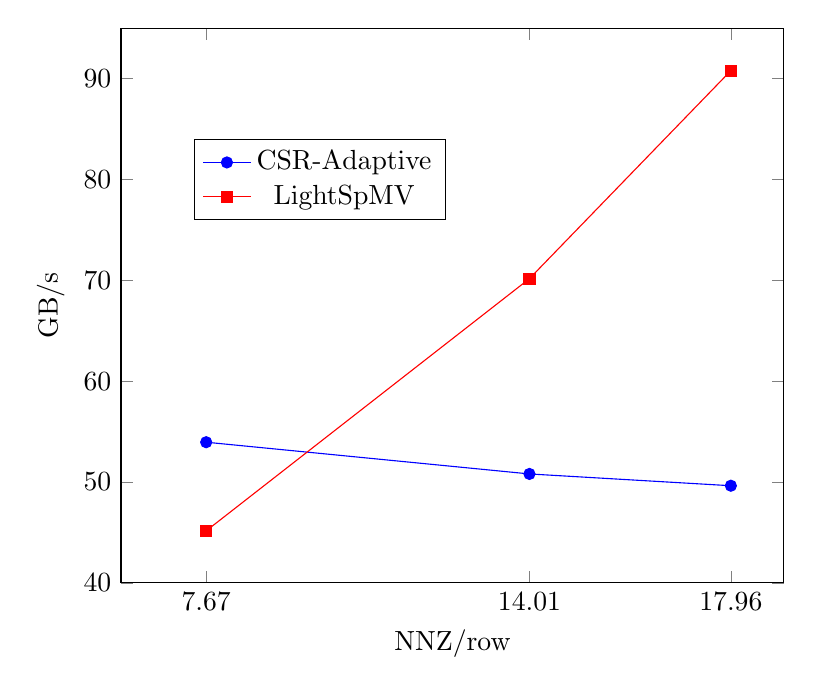
\begin{tikzpicture}
			\begin{axis}[        xlabel={NNZ/row},        ylabel={GB/s},        xmin=6, xmax=19,        ymin=40, ymax=95,        xtick={7.67,14.01,17.96},        legend style={at={(0.3,0.8)},anchor=north},        ]
				\addplot[color=blue,mark=*] coordinates {
					(7.67,53.944108)
					(14.01,50.797288)
					(17.96,49.628232)
				};
				\addlegendentry{CSR-Adaptive}
				
				\addplot[color=red,mark=square*] coordinates {
					(7.67,45.154160)
					(14.01,70.166256)
					(17.96,90.792728)
				};
				\addlegendentry{LightSpMV}
				
			\end{axis}
		\end{tikzpicture}
		\caption{GB/s vs. NNZ/row (Double precision).}
		\label{fig:multiple_line}
	\end{figure}
	
	\clearpage
	
	\subsection{Bar Plot}
	
	The bar plot is usually used to show the value of different categories. Let's say if I have code using four different algorithms (A, B, C, D) computing $a \times x$ where a and x are matrices. The time taken by each algorithm can be represented by \autoref{fig:bar_plot}.
	
	\begin{figure}[htbp]
		\centering
		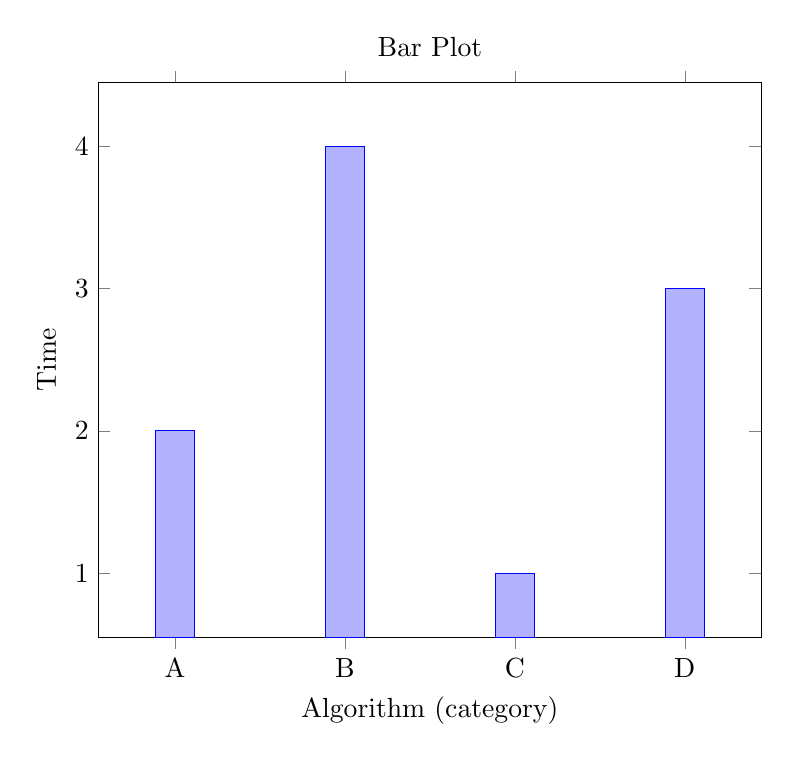
\begin{tikzpicture}
			\begin{axis}[
				xlabel = {Algorithm (category)},
				ylabel = {Time},
				title = {Bar Plot},
				symbolic x coords={A, B, C, D},
				ybar,
				bar width=0.5cm,
				enlargelimits=0.15,
				xtick=data,
				]
				\addplot coordinates {
					(A, 2)
					(B, 4)
					(C, 1)
					(D, 3)
				};
			\end{axis}
		\end{tikzpicture}
		\caption{Bar Plot}
		\label{fig:bar_plot}
	\end{figure}
	
	
	The stacked bar plot is used when each category also has sub-sections. Let's say if each algorithm has three parts and you want to also mention the time taken by each part in the same plot (\autoref{fig:stacked_ped}).
	
	
	\begin{figure}
		\centering
		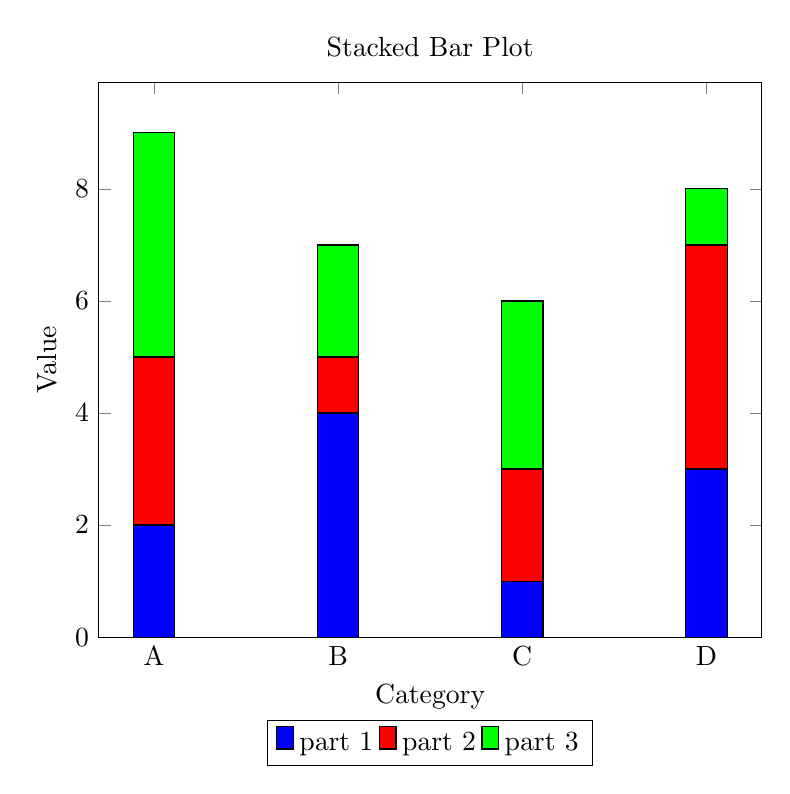
\begin{tikzpicture}
			\begin{axis}[
				xlabel = {Category},
				ylabel = {Value},
				title = {Stacked Bar Plot},
				ybar stacked,
				bar width=15pt,
				legend style={at={(0.5,-0.15)},
					anchor=north,legend columns=-1},
				symbolic x coords={A, B, C, D},
				xtick=data,
				ymin=0
				]
				\addplot [fill=blue] coordinates {
					(A, 2)
					(B, 4)
					(C, 1)
					(D, 3)
				};
				\addplot [fill=red] coordinates {
					(A, 3)
					(B, 1)
					(C, 2)
					(D, 4)
				};
				\addplot [fill=green] coordinates {
					(A, 4)
					(B, 2)
					(C, 3)
					(D, 1)
				};
				\legend{part 1, part 2, part 3}
			\end{axis}
		\end{tikzpicture}
		\caption{This is a stacked Bar Plot.}
		\label{fig:stacked_ped}
	\end{figure}
	
	
	In this example, the \codebox{ybar} stacked option is used to stack the bars vertically, and the bar width option is used to set the width of each bar. The symbolic x coords option is used to specify the categories on the x-axis. You can adjust the values, colors, labels, and other properties to fit your needs.
	
	Make sure you have the \codebox{pgfplots} package installed and included in your LaTeX environment for this code to work properly.
	
	\clearpage
	
	
	\subsection{Histogram}
	
	Histograms are commonly used in various fields for visualizing the distribution of data. Some areas where histograms are frequently employed include:
	
	\begin{itemize}
		\item Statistics: Histograms are widely used in statistical analysis to depict the frequency distribution of a dataset. They provide insights into the central tendency, spread, and shape of the data, allowing statisticians to make inferences and draw conclusions.
		
		\item Data Analysis: Histograms help analysts explore and understand the characteristics of a dataset. By examining the shape and peaks of the histogram, analysts can identify patterns, outliers, and potential data issues.
		
		\item Quality Control: Histograms play a vital role in quality control processes, especially in manufacturing industries. They are used to assess the distribution of measurements, identify process variations, and determine whether the produced items meet the required specifications.
		
		\item Market Research: In market research, histograms are employed to analyze survey responses, consumer preferences, and market trends. They aid in visualizing the distribution of responses, enabling researchers to gain insights into customer behavior and preferences.
		
		\item Image Processing: Histograms are utilized in image processing to enhance images and perform various operations such as contrast adjustment, equalization, and thresholding. They help analyze the distribution of pixel intensities within an image.
		
		\item Finance and Economics: In finance and economics, histograms are often used to examine the distribution of financial returns, market volatility, asset prices, and other economic indicators. They assist in understanding the risk and behavior of financial markets.
	\end{itemize} 
	
	These are just a few examples of the many areas where histograms are employed. Histograms provide a valuable tool for visualizing data distributions and are widely used across various domains for data exploration, analysis, and decision-making. \autoref{fig:his_ped} shows how to make one.
	
	\begin{figure}
		\centering
		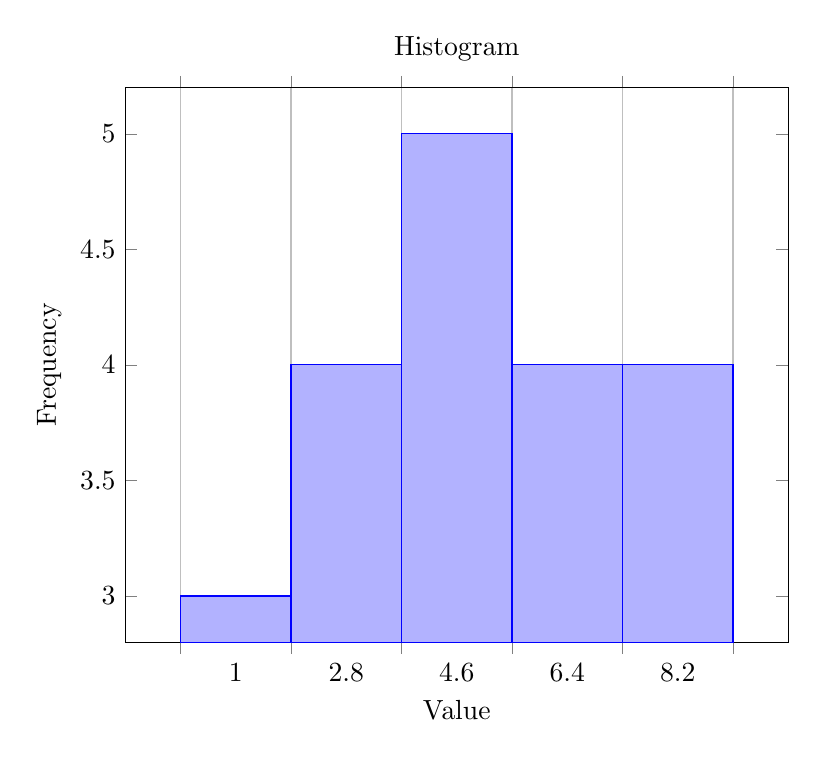
\begin{tikzpicture}
			\begin{axis}[
				xlabel = {Value},
				ylabel = {Frequency},
				title = {Histogram},
				ybar interval,
				xtick=data
				]
				\addplot+[hist={bins=5}] table[row sep=\\,y index=0] {
					data\\
					1\\ 2\\ 2\\ 3\\ 4\\
					4\\ 4\\ 5\\ 5\\ 5\\
					5\\ 6\\ 7\\ 7\\ 7\\
					8\\ 9\\ 9\\ 10\\ 10\\
				};
			\end{axis}
		\end{tikzpicture}
		\caption{This is a histogram.}
		\label{fig:his_ped}
	\end{figure}
	
	\clearpage
	
	\subsection{Pie Chart}
	
	Pie chart are used any time you want to show the percentages of items. To create a pie chart in LaTeX, you can use the \codebox{pgf-pie} package. Make sure you have it installed and then include the package in your LaTeX document (\autoref{fig:pie_pedram}):
	
	\begin{figure}[htbp]
		\centering
		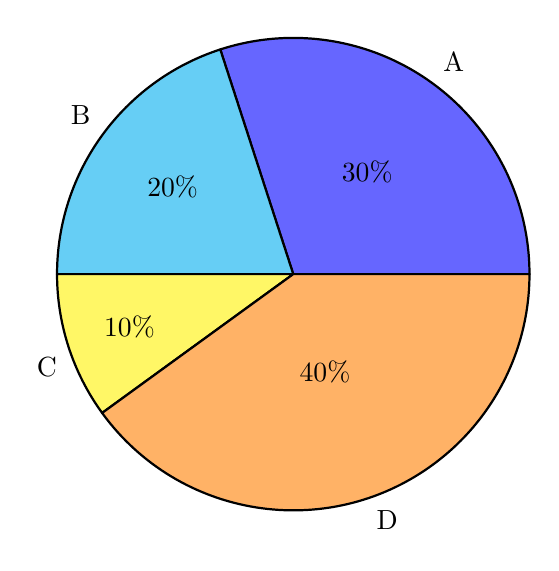
\begin{tikzpicture}
			\pie{30/A, 20/B, 10/C, 40/D}
		\end{tikzpicture}
		\caption{This is a pie Chart}
		\label{fig:pie_pedram}
	\end{figure}
	
	In this example, the placement options \codebox{[htbp]} are used within the figure environment. The options specify the preferred positions for the figure: h for "here", t for "top", b for "bottom", and p for "page" (a dedicated float page). The order of the options determines the priority for placement. Remove this option and compile you file to see the location of plot!
	
	In this example, the \codebox{pie} command is provided by the pgf-pie package, which creates a pie chart. Each slice of the pie is represented by a percentage value followed by a label. You can adjust the values and labels according to your needs.
	
	Make sure you have the \codebox{pgf-pie} package installed and included in your LaTeX environment for this code to work properly.
	
	
	\subsection{Box Plot}
	
	This plot is usually used in Data Science. To create a box plot in LaTeX using pgfplots, you can use the statistics library by including \codebox{\textbackslash usetikzlibrary\{pgfplots.statistics\}} at before \codebox{\textbackslash begin\{document\}}.
	
	
	\begin{figure}
		\centering
		\begin{tikzpicture}
			\begin{axis}[
				title = {Box Plot},
				ylabel = {Value},
				boxplot/draw direction=y
				]
				\addplot+[
				boxplot prepared={
					median=5,
					upper quartile=7,
					lower quartile=3,
					upper whisker=10,
					lower whisker=2
				}
				] coordinates {};
			\end{axis}
		\end{tikzpicture}
		\caption{Box Plot}
	\end{figure}
	
	\begin{tcolorbox}[myboxstyle]
		
		{\Large \textbf{\textcolor{cherry}{Tips!}}} These are only few examples of chart, you can always ask chatGPT based on your problem to give you some samples. Make sure if you are working for a company, you are not sharing sensitive information with ChatGPT. Give it some sample data not the real one! 
		
	\end{tcolorbox}
	
	\clearpage
	
	
	
	
	
	
	
	\section{C Code Box or Inline}
	
	To include C code in your LaTeX document, you have two options: using a code box or including code inline.
	
	\subsection{Code Box}
	
	To display a block of C code with syntax highlighting and line numbers, you can use the \codebox{lstlisting} environment from the \codebox{listings} package. Here's an example:
	
	\begin{lstlisting}[language=C, caption={Example of C code in a code box}]
		#include <stdio.h>
		int main() {
			printf("Hello, McMaster!\n");
			return 0;
		}
	\end{lstlisting}
	
	In this example, the \codebox{language} option is set to \codebox{C} to enable C language syntax highlighting. The \codebox{caption} option is used to provide a descriptive caption for the code box.
	
	\subsection{Inline Code}
	
	To include a small snippet of C code inline with your text, you can use the \codebox{\textbackslash codebox\{\}} command. Here's an example:
	
	\codebox{printf("Hello LaTeX")}
	
	Remember to include the necessary packages in the preamble of your LaTeX document, such as \codebox{\textbackslash usepackage\{listings\}} for code formatting and syntax highlighting.
	
	Compile the LaTeX code to see the C code box and inline code snippet rendered in your document.
	
	
	\begin{tcolorbox}[myboxstyle]
		
		{\Large \textbf{\textcolor{cherry}{More details!}}} You don't need to know how
		
		\codebox{\textbackslash codebox\{\}}
		
		and
		
		\codebox{\textbackslash begin\{lstlisting\} ... \textbackslash end\{lstlisting\}}
		
		work in this course. You need to just be able to use it and make your documentation. But if your are interested, especially I am sure in future you will need to know it, the following description gives you more details.
		
	\end{tcolorbox}
	
	\begin{enumerate}
		\item \textbf{Code box}: The lstlisting environment is part of the listings package in LaTeX, which provides a way to include code listings in your documents. You can make a default format for your lstlisting, for example:
		
		\begin{lstlisting}
			\lstset{
				language=C,
				basicstyle=\ttfamily,
				backgroundcolor=\color{blue!5},
				keywordstyle=\color{blue},
				commentstyle=\color{codegreen},
				stringstyle=\color{red},
				showstringspaces=false,
				breaklines=true,
				frame=single,
				rulecolor=\color{lightgray!35},
				numbers=none,
				numberstyle=\tiny,
				numbersep=5pt,
				tabsize=1,
				alsoletter={\#},
				otherkeywords={\#}
			}
			
		\end{lstlisting}    
		
		\begin{itemize}
			\item \codebox{language=C}: Sets the language for syntax highlighting. In this case, it is set to C. You can change it to match the desired language or remove this line if you don't want syntax highlighting.
			
			\item \codebox{basicstyle=\textbackslash ttfamily}: Sets the basic style for the code listing. \codebox{\textbackslash ttfamily} selects a monospaced font, suitable for code.
			
			\item \codebox{backgroundcolor=\textbackslash color\{blue!5\}}: Sets the background color for the code listing. In this example, it is set to a light blue color with a transparency of 5\%.
			
			\item \codebox{keywordstyle=\textbackslash color\{blue\}}: Sets the color for keywords in the code. In this example, keywords will be displayed in blue.
			
			\item \codebox{commentstyle=\textbackslash color\{codegreen\}}: Sets the color for comments in the code. In this example, comments will be displayed in a custom color named codegreen.
			
			\item \codebox{stringstyle=\textbackslash color\{red\}}: Sets the color for strings (e.g., text within quotation marks) in the code. In this example, strings will be displayed in red.
			
			\item \codebox{showstringspaces=false}: Specifies whether to show spaces within strings. In this example, spaces within strings will not be visible.
			
			\item \codebox{breaklines=true}: Allows automatic line breaking if a line of code exceeds the width of the listing. This ensures that the code fits within the specified frame.
			
			\item \codebox{frame=single}: Adds a frame around the code listing. In this example, a single line frame will be displayed.
			
			\item \codebox{rulecolor=\textbackslash color\{lightgray!35\}}: Sets the color for the frame of the code listing. In this example, the frame color is a light gray with a transparency of 35\%.
			
			\item numbers=none: Disables line numbering for the code listing.
			
			\item \codebox{numberstyle=\textbackslash tiny}: Sets the style for line numbers. In this example, line numbers will be displayed in a tiny font size.
			
			\item \codebox{numbersep=5pt}: Specifies the distance between line numbers and the code.
			
			\item \codebox{tabsize=1}: Sets the tab size for indentation. In this example, each tab will be equivalent to one character width.
			
			\item \codebox{alsoletter={\textbackslash \#}}: Specifies additional characters that should be treated as letters. In this example, the \# symbol is included.
			
			\item \codebox{otherkeywords={\textbackslash \#}}: Specifies additional keywords. In this example, the \# symbol is included as a keyword.
			
		\end{itemize}
		
		These settings can be defined in the preamble of your LaTeX document, or you can define them locally within a specific lstlisting environment.
		
		To use the listings package, you need to include the following line in your LaTeX document's preamble: \codebox{\textbackslash usepackage\{listings\}}. After including this package the mentioned settings will be added before \codebox{\textbackslash begin\{document\}}. 
		
		Additionally, you may need to load other packages depending on the colors and symbols used. In the provided example, the code assumes the usage of the color package to define custom colors. You can include the following line in your preamble to load it: \codebox{\textbackslash usepackage\{xcolor\}}. 
		
		Make sure to have both the listings and xcolor packages installed in your LaTeX environment to use the provided settings.
		
		
		\item \textbf{Inline Code}: Here I have defined a new environment called \textbf{codebox}. This a name I chose to remember during writing, you can choose any thing. and I can use it during writing by \codebox{\textbackslash codebox\{\}}. This is how I have defined the environment before \codebox{\textbackslash begin\{document\}}:
		
		\begin{lstlisting}
			\newtcbox{\codebox}[1][gray]{on line, boxrule=0.2pt, colback=blue!5, colframe=#1, fontupper=\color{cherry}\ttfamily, arc=2pt, boxsep=0pt, left=2pt, right=2pt, top=3pt, bottom=2pt}
		\end{lstlisting}
		
		\begin{itemize}
			\item \codebox{\textbackslash newtcbox}: This command is used to define a new box environment named \textbackslash codebox. It creates a colored and rounded box to display inline code snippets.
			
			\item \codebox{\textbackslash codebox}: This is the name of the defined box environment, which can be used to wrap inline code snippets.
			
			\item \codebox{[1][gray]}: This optional parameter allows you to specify the color of the box frame. By default, if no color is specified, the box frame will be gray.
			
			\item \codebox{on line}: This option specifies that the box should be placed on the same line as the text.
			
			\item \codebox{boxrule=0.2pt}: This sets the thickness of the box's frame.
			
			\item \codebox{colback=blue!5}: This defines the background color of the box. In this example, it is set to a light blue with a transparency of 5\%.
			
			\item \codebox{colframe=\#1}: This sets the color of the box's frame. The \#1 parameter refers to the optional parameter passed when using \textbackslash codebox, allowing you to customize the frame color.
			
			\item \codebox{fontupper=\textbackslash color\{cherry\}\textbackslash ttfamily}: This sets the font style for the text inside the box. It uses the color cherry (which should be defined elsewhere) and a monospaced font (\codebox{\textbackslash ttfamily}) to display the code.
			
			\item \codebox{arc=2pt}: This sets the radius of the rounded corners of the box.
			
			\item \codebox{boxsep=0pt}: This sets the spacing between the text and the box's frame.
			
			\item \codebox{left=2pt, right=2pt, top=3pt, bottom=2pt}: These options define the padding (space) around the text within the box. You can adjust these values to change the amount of padding.
			
		\end{itemize}
		
		You can use the \codebox{\textbackslash codebox} command to wrap inline code snippets and display them with a colored and rounded box.
		
		Make sure to define the necessary colors (cherry in this case) and load the required packages (tcolorbox, if not already loaded) in the preamble of your LaTeX document for the \codebox{\textbackslash newtcbox} command to work properly.
		
	\end{enumerate}
	
	
	
	
	
	\section{Tables of Contents} \label{sec:TOC}
	
	You can customize the appearance of \codebox{section},  \codebox{subsection}, and  \codebox{subsubsection} headings, as well as the entries in the table of contents (TOC) for these sections. At the top of this file we have:
	
	\begin{lstlisting}[style=latexstyle]
		% Set the color for the section headings
		\titleformat{\section}
		{\normalfont\Large\bfseries\color{orange!80!black}}{\thesection}{1em}{}
		
		% Set the color for the subsection headings
		\titleformat{\subsection}
		{\normalfont\large\bfseries\color{orange!80!black}}{\thesubsection}{1em}{}
		
		% Set the color for the subsubsection headings
		\titleformat{\subsubsection}
		{\normalfont\normalsize\bfseries\color{orange!80!black}}{\thesubsubsection}{1em}{}
	\end{lstlisting}
	
	Here's a breakdown of what each part does:
	
	\begin{itemize}
		\item \codebox{\textbackslash titleformat\{\textbackslash section\}}: Modifies the appearance of section headings.
		\item \codebox{\textbackslash titleformat\{\textbackslash subsection\}}: Modifies the appearance of subsection headings.
		\item \codebox{\textbackslash titleformat\{\textbackslash subsubsection\}}: Modifies the appearance of subsubsection headings.
	\end{itemize}
	
	For each of the above the part \codebox{\textbackslash normalfont\textbackslash Large\textbackslash bfseries\textbackslash color\{orange!80!black\}}:
	
	\begin{itemize}
		\item \codebox{\textbackslash Large}: Sets the font size to "large".
		\item \codebox{\textbackslash bfseries}: Makes the text bold.
		\item \codebox{\textbackslash color\{orange!80!black\}}: Sets the text color to a mix of 80\% orange and 20\% black.
	\end{itemize}

	\codebox{\textbackslash tableofcontents} is a command in LaTeX used to generate the table of contents (TOC) based on the document's sectioning commands (such as \codebox{\textbackslash section}, \codebox{\textbackslash subsection}, etc.) and their associated titles. You can modify how the table looks like by:
	
	\begin{lstlisting}[style=latexstyle]
		% Set the color for the table of contents
		\titlecontents{section}
		[1.5em]{\color{orange!80!black}}
		{\contentslabel{1.5em}}
		{}{\titlerule*[0.5pc]{.}\contentspage}
		
		% Set the color for the subsections in the table of contents
		\titlecontents{subsection}
		[3.8em]{\color{orange!80!black}}
		{\contentslabel{2.3em}}
		{}{\titlerule*[0.5pc]{.}\contentspage}
		
		% Set the color for the subsubsections in the table of contents
		\titlecontents{subsubsection}
		[6em]{\color{orange!80!black}}
		{\contentslabel{3em}}
		{}{\titlerule*[0.5pc]{.}\contentspage}
	\end{lstlisting}
	
	
	Here's a breakdown of what each part does:
	
	\begin{itemize}
		\item \codebox{\textbackslash titlecontents\{section\}}: Customizes the appearance of section entries in the table of contents.
		\item \codebox{\textbackslash titlecontents\{subsection\}}: Customizes the appearance of subsection entries in the TOC.
		\item \codebox{\textbackslash titlecontents\{subsubsection\}}: Customizes the appearance of subsubsection entries in the TOC.
	\end{itemize}
	
	
	
	For each of the TOC entries:
	
	\begin{itemize}
		
		\item \codebox{[1.5em]}, \codebox{[3.8em]}, \codebox{[6em]}: Adjusts the horizontal space allocated for the entry label.
		
		\item \codebox{\textbackslash color\{orange!80!black\}}: Sets the color of the TOC entry text to a mix of 80\% orange and 20\% black.
		
		\item \codebox{\textbackslash contentslabel\{1.5em\}}, \codebox{\textbackslash contentslabel\{2.3em\}}, \codebox{\textbackslash contentslabel\{3em\}}: Sets the indentation of the label in the TOC.
		
		\item \codebox{\textbackslash titlerule*[0.5pc]\{.\}\textbackslash contentspage}: Specifies the formatting of the entry, including vertical spacing, horizontal rule, and page numbers.
	\end{itemize}
	
	Overall, this code snippet is used to customize the appearance of sectioning headings (section, subsection, subsubsection) and their corresponding entries in the table of contents by changing their font size, weight (boldness), and color. Adjustments are made to their label indentation and formatting within the TOC as well.
	
	
	
	Also, you can customize the header and footer styles for the pages in your document using:
	
	
	\begin{lstlisting}[style=latexstyle]
		% Apply the custom footer to all pages
		\pagestyle{fancy}
		
		% Redefine the header format
		\fancyhead{}
		\fancyhead[R]{\textcolor{orange!80!black}{\itshape\leftmark}}
		
		\fancyhead[L]{\textcolor{black}{\thepage}}
		
		
		% Redefine the footer format with a line before each footnote
		\fancyfoot{}
		\fancyfoot[C]{\footnotesize P. Pasandide, McMaster University, Computer Science Practice and Experience: Development Basics. \footnoterule}
		
		% Redefine the footnote rule
		\renewcommand{\footnoterule}{\vspace*{-3pt}\noindent\rule{0.0\columnwidth}{0.4pt}\vspace*{2.6pt}}
		
		% Set the header rule color to orange
		\renewcommand{\headrule}{\color{orange!80!black}\hrule width\headwidth height\headrulewidth \vskip-\headrulewidth}
		
		% Set the footer rule color to orange (optional)
		\renewcommand{\footrule}{\color{black}\hrule width\headwidth height\headrulewidth \vskip-\headrulewidth}
	\end{lstlisting}
	
	
	Here's a breakdown of each command:
	
	\begin{itemize}
		\item \codebox{\textbackslash pagestyle\{fancy\}}: Applies the custom page style fancy to all pages. This style allows the customization of headers and footers.
		
		\item \textbf{Header Formatting}:
		\begin{itemize}
			\item \codebox{\textbackslash fancyhead\{\}}: Clears the default header settings.
			\item \codebox{\textbackslash fancyhead[R]\{\textbackslash textcolor\{orange!80!black\}\{\textbackslash itshape\textbackslash leftmark\}\}}: Sets the right-side header to display the section name (using \codebox{\textbackslash leftmark}) in italic font and orange color (\codebox{orange!80!black}).
			\item \codebox{\textbackslash fancyhead[L]\{\textbackslash textcolor\{black\}\{\textbackslash thepage\}\}}: Sets the left-side header to display the page number in black.
		\end{itemize}
	
		\item \textbf{Footer Formatting}:
		
		\begin{itemize}
			\item \codebox{\textbackslash fancyfoot\{\}}: Clears the default footer settings.
			\item \codebox{\textbackslash fancyfoot[C]\{\textbackslash footnotesize ...\}}: Sets the center part of the footer to display a customized footnote text, including author, university, and a publication reference.
		\end{itemize}
		

		\item \textbf{Footer Rule Customization}:
		\begin{itemize}
			\item \codebox{\textbackslash renewcommand\{\textbackslash footnoterule\}\{...\}}: Redefines the format of the rule before footnotes, adjusting its width, height, and spacing.
			\item \codebox{\textbackslash renewcommand\{\textbackslash headrule\}\{...\}}: Redefines the header rule's color to orange (orange!80!black) and sets its width and height.
			\item \codebox{\textbackslash renewcommand\{\textbackslash footrule\}\{...\}}: Optionally sets the footer rule color to black (black) and adjusts its width, height, and spacing.
		\end{itemize}
		
	\end{itemize}

	This block of code establishes a custom page style (\codebox{fancy}) and sets specific formatting for headers and footers. It defines rules and footnotes' appearance, utilizing colors, widths, heights, and text styles to create a distinctive header and footer design across all pages of your document. Adjustments can be made to these settings to suit your desired layout and styling preferences.
	

	
	\section{Reference} \label{sec:Reference}
	

	Here's an overview of referencing methods in LaTeX that so far we worked with:
	
	\begin{enumerate}
		\item \codebox{\textbackslash href\{URL\}\{text\}}
		
		\begin{itemize}
			\item Purpose: Creates a hyperlink to an external URL.
			\item Usage: \codebox{\textbackslash href\{URL\}\{text\}} creates a clickable link to an external website.
			\item Example: \href{https://github.com/pedrampasandide1993}{My GitHub} generates a link to my github.
		\end{itemize}
		
		\item \codebox{\textbackslash hyperref[label]\{text\}}
		
		\begin{itemize}
			\item Purpose: Creates an internal hyperlink within the document.
			\item Usage: \codebox{\textbackslash hyperref[label]\{text\}} references a labeled part within the same document.
			\item Example: \hyperref[sec:TOC]{Table of Contents} links to a section labeled as "sec:TOC."
		\end{itemize}

		\item \codebox{\textbackslash autoref\{label\}}
		
		\begin{itemize}
			\item Purpose: Automatically generates references with context.
			\item Usage: \codebox{\textbackslash autoref\{label\}} generates references to figures, tables, sections, etc., adding the appropriate label (e.g., "Figure," "Table") and its number.
			\item Example: \autoref{fig:scatter_pedram} references a figure labeled as "fig:scatter\_pedram."
		\end{itemize}
		

	\end{enumerate}
	
	These referencing methods allow you to create both internal and external links within your LaTeX document, referencing various elements like websites, internal document sections, figures, tables, etc. \codebox{\textbackslash autoref} specifically generates references with appropriate labels and numbers based on the referenced element type. Adjust labels and text to match the specific content and structure of your document.
	
	
	Sometimes you want to refer to an article or published paper. Using \codebox{\textbackslash cite\{\}} for scientific referencing involves several steps:
	
	\textbf{Step 1: Document Setup}
	
	Document Class: Choose a document class that supports bibliography and citations, such as \codebox{article}, \codebox{report}, or \codebox{book}.
	
	Bibliography Style: Select a bibliography style (e.g.,\codebox{plain}, \codebox{IEEEtran}, \codebox{apa}) using the \codebox{\textbackslash bibliographystyle\{\}} command.
	
	\textbf{Step 2: Insert Citations}
	
	Create a Bibliography File: Start by creating a separate \codebox{.bib} file (e.g., \codebox{nano references.bib}) to store your bibliography entries.
	
	Add Citations: Inside the \codebox{.bib} file, add entries for each reference in BibTeX format. For example:
	
	\begin{lstlisting}
		@article{PASANDIDE202130005,
			title = {Simulation and optimization of continuous catalytic reforming: Reducing energy cost and coke formation},
			journal = {International Journal of Hydrogen Energy},
			volume = {46},
			number = {58},
			pages = {30005-30018},
			year = {2021},
			issn = {0360-3199},
			doi = {},
			url = {},
			author = {Pedram Pasandide and Mohammad Rahmani},
			abstract = {}
		}
	\end{lstlisting}
	
	Google on how you can get \codebox{.bib} format of an article or a book!
	
	
	\textbf{Step 3: Incorporate Citations in Document}
	
	Cite References: Within your LaTeX document, use \codebox{\textbackslash cite\{\}} to reference these entries.
	

	
	Insert Bibliography: Use \codebox{\textbackslash bibliography\{\}} to specify the \codebox{.bib} file and \codebox{\textbackslash bibliographystyle\{\}} to set the bibliography style. For example:
	
	\begin{lstlisting}[basicstyle=\small]
		\bibliography{references} % Replace 'references' with your .bib file name
		\bibliographystyle{plain} % Replace 'plain' with the style you prefer
	\end{lstlisting}
	
	For instance:
	
	\begin{lstlisting}[basicstyle=\footnotesize]
		\documentclass{article}
		
		\begin{document}
			
			
			Example: \cite{PASANDIDE202130005} will cite the Pasandide (2021) article.
			\bibliographystyle{plain}
			\bibliography{references} % Replace 'references' with your .bib file name
			
		\end{document}
		
	\end{lstlisting}
	
	Make sure to replace references with the actual name of your .bib file and update \codebox{\textbackslash cite\{\}} with the appropriate citation keys from your bibliography. Then, follow the compilation steps mentioned above to generate the bibliography in your document.
	
	Example: \cite{PASANDIDE202130005} will cite the Pasandide (2021) article.
	
%	\pdftooltip{\href{https://www.google.com/search?channel=fs&client=ubuntu-sn&q=is+excel+vba+a+programming+language}{%
%			\includegraphics[width=0.8\linewidth]{instagram_post_image.jpg} % Replace 'instagram_post_image.jpg' with the image of the post
%	}}{%
%		A post shared by Instatus (@instatushq) % Caption of the Instagram post
%	}
%	
%	
%	\includegraphics[width=0.8\linewidth]{Instagram_logo_2022.jpg}

	\bibliographystyle{plain}
	\bibliography{references} % Replace 'references' with your .bib file name
	
	
	
	
	\clearpage
	
\end{document}